
As we are working with open source tools we decided to license our project using the MIT License. MIT License is a permissive license and one of the most used open source licenses. It allows the public to modify, share and for commercial use without us being liable for anything. To decide on the license we analyzed our goals for this project which is to have future contributions as well as help others on their work just as we got inspired by the ITU-MiniTwit before the refactoring process. In terms of license compatibility, our top-level dependencies falls into the MIT and Apache 2.0 licenses which a both permissive open source solution high compatible. See Figure\ref{fig:license}.
\begin{figure}[h]
    \centering
    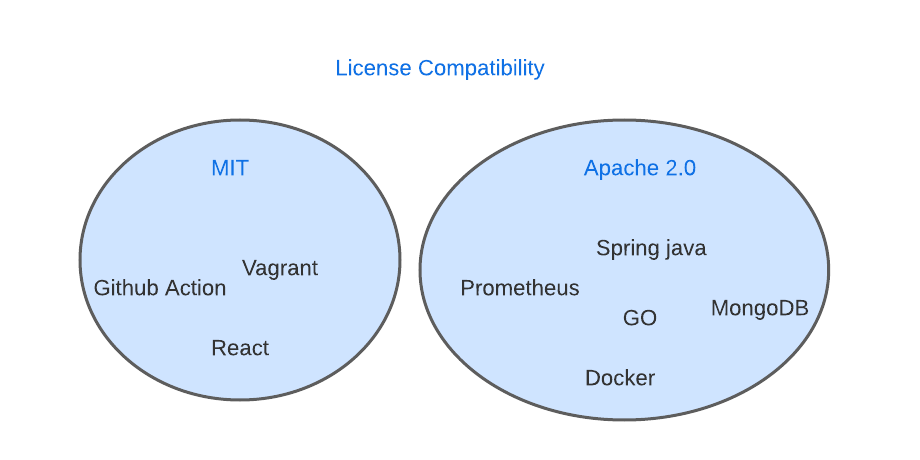
\includegraphics[width = .7\textwidth]{images/License.png}
    \caption{License Distribution}
    \label{fig:license}
\end{figure}